% !TEX root = ../notes.tex

% ================  (Interactive) Visualization ==============

\section{Supervised Learning}

%=============================================
\subsection{Introduction to Machine Learning}

{\bf Machine Learning} is an extended field characterized by many facets. The  \href{https://en.wikipedia.org/wiki/Arthur\_Samuel}{Arthur Samuel}'s definition can be considered the most meaningful one: ``{\it Field of study that gives computers the ability to learn without being explicitly programmed.}''. The aim of \emph{Machine Learning} is to model into a computer the learning and adapting procedures that characterize the human way of thinking and processing information. Merely, the idea behind is to use computers to apply statistical and optimization algorithms to \emph{automatically} identify pattern in data and/or classify them. 

To get an idea of what \emph{Machine Learning} does and consists of, take a look at a \href{http://www.r2d3.us/visual-intro-to-machine-learning-part-1/}{beautiful introduction to Machine Learning}. In order to capture the essence of this subject, it speaks more than thousand words . 

In the end, according to a reductive point of view, we may simply say that Machine Learning is born because we are \textbf{lazy} and we let the machine do the ``work'' for us. 
\\\\
\emph{Machine Learning} is based on the definition of algorithms that allows the aforementioned procedures. Those algorithms can be distinguished either by the \emph{learning style} (Supervised vs Unsupervised vs Semi-Supervised learning) or by their \emph{similarity}. 

In the next part of this chapter, we first give an introduction to \emph{Supervised} and \emph{Unsupervised} learning and then we go deeper into \emph{Supervised Learning}. If you want to become a Machine Learning Master, you should have a look \href{http://machinelearningmastery.com/}{here}.

%=============================================
\subsubsection{Different aspects of Machine Learning} 

When we apply a \emph{Machine Learning} method, one on the thing that we are mostly interested in is getting good predictions. This is not the only important aspect of the Machine Learning methods though. 

The following list rough out some very important aspects for these methods:

\begin{itemize}
\item \textbf{Predictive accuracy}: we want our model to return correct result;
\item \textbf{Speed and scalability}: the model should be efficient in order to be easily applied
  \begin{itemize}
   \item Time to build the model
   \item Time to use the model
   \item In memory vs Disk processing
  \end{itemize}
\item \textbf{Robustness}: the method should not be too sensitive
  \begin{itemize}
   \item Handling noise
   \item Handling outliers
   \item Handling missing values
  \end{itemize}
\item \textbf{Interpretability}
  \begin{itemize}
   \item Understand the model and its decisions (\emph{black box} vs {white box})
   \item Compactness of the model
  \end{itemize}
\end{itemize}

%=============================================
\subsubsection{Supervised vs Unsupervised Learning}

In Table \ref{tab:sup-unsup} we outline some differences/similarities between \emph{Supervised} and \emph{Unsupervised} learning. 

The main difference to remark is that for \emph{Supervised} learning, we use a \emph{training} data with \textbf{known} labels and we test it on a\emph{test} data \textbf{without} labels. For \emph{Unsupervised} learning we do not have any labels. We are just trying to simplify/cluster the samples.

\begin{table}[h!]
  \centering
  \begin{tabular}{m{2cm}||m{5.5cm}|m{5.5cm}}
    & \textbf{Supervised} & \textbf{Unsupervised} \\ \hline\hline
    \textbf{Variables} & Samples $X$ and labels $y$ & Samples $X$ \\ \hline
    \textbf{Learning} & Function $y = f(X)$ relate samples and labels. We would like to ``learn'' $f$ and evaluate it on new data. & We want to compute a function $y = f(X)$ to give a \emph{simpler} representation of the samples X. \\ \hline
    \textbf{Discrete \newline labels} & {\bf Classification} & {\bf Clustering} \\ \hline
    \textbf{Continuous labels} & Regression & Matrix factorization, Kalman filtering, Unsupervised neural networks \\ \hline 
    \text{Examples} & 
	      $\bullet$ Is this image a cat, dog, car, house? \newline
	      $\bullet$ How would this user score that restaurant? \newline
	      $\bullet$ Is this email spam? \newline
	      $\bullet$ Is this blob a supernova?
	     &
	      $\bullet$ Cluster some hand-written digit data into 10 classes. \newline
	      $\bullet$ What are the top 20 topics in Twitter right now? \newline
	      $\bullet$ Find and cluster distinct accents of people in Lausanne
            \\ \hline
    \textbf{Techniques} & 
	      $\bullet$ k Nearest Neighbors \newline
	      $\bullet$ Na\"ive Bayes \newline
	      $\bullet$ Linear + Logistic Regression \newline
	      $\bullet$ Support Vector Machines \newline
	      $\bullet$ Random Forests \newline
	      $\bullet$ Neural Networks
	    &
	      $\bullet$ Clustering \newline
	      $\bullet$ Topic Models \newline
	      $\bullet$ Hidden Markov Models
	    \\ \hline
  \end{tabular}
  \label{tab:sup-unsup}
  \caption{Summary of the differences between Supervised and Unsupervised learning.}
\end{table}

%=============================================
\subsection{More details on Supervised Learning}

%=============================================
\subsubsection{Predicting from Samples}

The \textbf{samples} are, most of the time, subsets of an infinite population. We are interested in a model that can {\bf describe the whole population}, but since we only have access to a \emph{sample} of it, it is not possible. Therefore we train on a training sample $D$ and we denote the model found by $f_D(X)$, $X$ being the features.
Most of the datasets are \textbf{samples} from an infinite population, \emph{i.e.} a subset of an \textbf{infinite} dataset. We would like to model the \textbf{whole population}, but only have access to a sample of it. So, we train on a training sample called $D$ and we denote the model as $f_D(X)$ where $X$ are the features and $y=f_D(X)$ the predictions.

%=============================================
\subsubsection{Bias and Variance}

The data-generated model $f_D(X)$ is a \textbf{statistical estimate} of the true function $f(X)$ (function working for the whole population). Therefore the model is subject to bias and variance. 
\\
The \textbf{Bias} is defined as the \emph{expected difference} between the prediction of a model $f_D(X)$ and the true labels $y$:
\[
 \textrm{Bias} = \mathbb{E}\left[ f_D(X)-y\right]
\]
\\
The \textbf{Variance} is defined as:
\[
 \textrm{Variance} = \mathbb{E}\left[\left(f_D(X) - \overline{f}(X)\right)^2\right]
\]
where $\overline{f}(X) = \mathbb{E}\left[f_D(X)\right]$ being the average prediction on X.

Bias and Variance are very useful to understand if you are doing something wrong. Thus, it is important to understand what you are doing and not just applying ``black-boxed'' algorithms.

\subsubsection*{ Trade-off between Bias and Variance}

The \href{http://scott.fortmann-roe.com/docs/BiasVariance.html}{tradeoff between bias and variance} is due to model complexity, see Figure \ref{fig:simple_complex}.
\begin{itemize}
 \item \textbf{Complex models}: Many parameters, usually lower bias (the model is close to the model that generates the data) but higher variance (the predictions have high variability). It leads to the risk of overfitting. Merely, this kind of models describe well the sample population, likely they do not represent well the entire population though.
 \item \textbf{Simple models}: Few parameters, higher bias (far from the true model) but lower variance (less variability among predictions), It may ends up with the underfitting.
\end{itemize}
\begin{figure}[H] %----------- Graph ---------------------
\centerline{
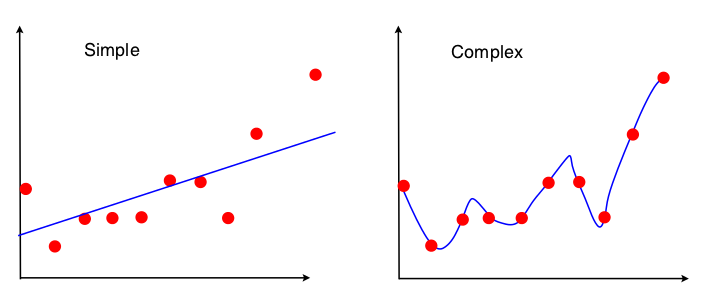
\includegraphics[width=13cm]{img/07/simple_complex}
}
\caption{\label{fig:simple_complex} 
Illustrations of a simple model and a complex model on the same data.
}
\end{figure}


For example, a linear model can only fit a straight line. A high degree polynomial can fit complex curves. Therefore this polynomial will work very well with the samples but not that well with the whole population. Thus a high variance is expected.
\\\\
In order to take into account this trade-off, we introduce the total expected error is 
\[
 \textrm{Bias}^2 + \textrm{Variance}
\]
This error {\bf balance} the contributions of the variance and the bias. 

\begin{figure}[H] %----------- Graph ---------------------
\centerline{
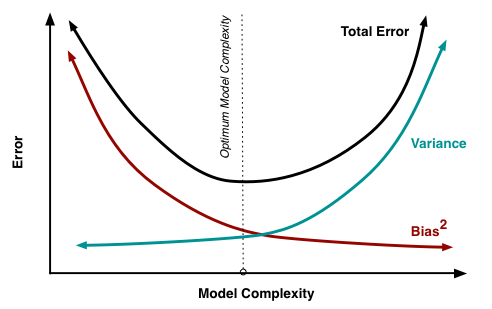
\includegraphics[width=10cm]{img/07/biasvariance}
}
\caption{\label{BV} 
Illustration of the model complexity and the Bias Variance tradeoff. The optimum model complexity is when the total error is minimized.
}
\end{figure}
When the Bias and the Variance are unbalanced, we use the terms:
\begin{itemize}
 \item {\bf overfitting} when the \emph{Variance} strongly dominates. (Too much variation between models. Hence, the model does not work well on new data)
 \item {\bf underfitting} when the \emph{Bias} strongly dominates. (The models do not fitting the data well enough)
\end{itemize}


%=============================================
\subsection{k-Nearest Neighbors}

The kNN algorithm is a well known method used for classification and regression. Given a  query item, the idea of the kNN algorithm is to find the \emph{k} nearest neighbors (\emph{k} closest matches) using a specific metric. Once we found them, we label the item such that it corresponds to the most frequent label in the neighbors. Figure \ref{fig:knn} shows an example with cats and other animals.

\begin{figure}[H] %----------- Graph ---------------------
\centerline{
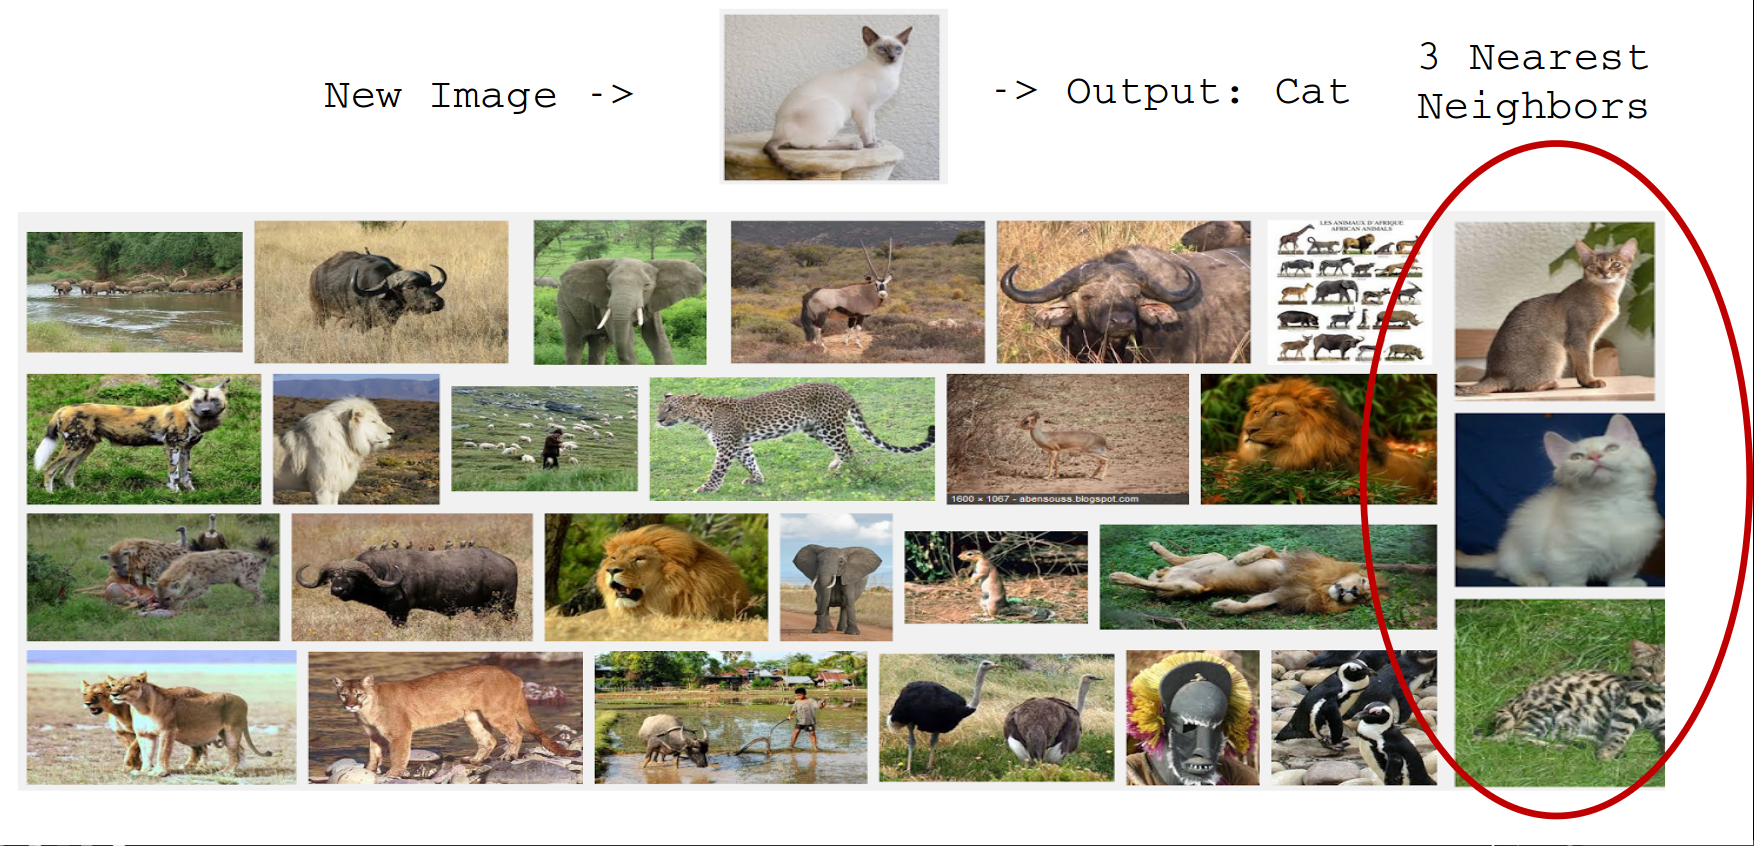
\includegraphics[width=13cm]{img/07/knn}
}
\caption{\label{fig:knn} 
Illustration of the kNN algorithm.
}
\end{figure}

However, this very simple algorithm has one issue: the Data {\bf is} the Model. This implies:
\begin{itemize}
 \item No training needed.
 \item The accuracy generally improves with more data.
 \item Matching is simple and fairly fast if data fits in memory. (Can be run off disk)
\end{itemize}
Normally, the only parameter is $k$, the number of neighbors. But two other choices are important:
\begin{itemize}
 \item Weighting of neighbors (e.g. inverse distance)
 \item Similarity metric.
\end{itemize}

%=============================================
\subsubsection{kNN Flavors}
The kNN algorithm can be used both for regression and classification. Table \ref{tab:knn} gives the similarities/differences of the kNN algorithm for regression and classification.
\begin{table}[h!]
 \centering
 \begin{tabular}{p{7cm}|p{7cm}}
  \textbf{Classification} & \textbf{Regression} \\ \hline \hline
  The model is $y=f(X)$ where $y$ is from a discrete set (labels). & The model is $y=f(X)$ where $y$ is a real value. \\ \hline
  Given $X$, we compute $y$ being the majority vote of the k nearest neighbors. & Given $X$, we compute $y$ being the average value of the k nearest neighbors. \\ \hline
  We can also use a weighted vote of the neighbors. & We can also use a weighted average of the neighbors.
 \end{tabular}
 \label{tab:knn}
 \caption{kNN algorithm used for classification and regression: Differences and similarities. Usually, the weight function is the inverse distance. 
}
\end{table}

%=============================================
\subsubsection{kNN distance measures}
For the kNN algorithm, we need to use a distance between the neighbors. The choice of the distance function can be very different depending on what you are looking for. We give here some examples:
\begin{description}
 \item[Euclidean distance]: Simple and fast to compute.
 \[
  d(x,y) = ||x-y||
 \]

 \item[Cosine Distance]: Good for documents, images, etc.
 \[
  d(x,y) = 1- \frac{x\cdot y}{||x||||y||}
 \]

 \item[Jaccard Distance]: For set data
 \[
  d(X,Y) = 1 - \frac{|X \cap Y|}{|X \cup Y|}
 \]

 \item[Hamming Distance]: For string data
 \[
  d(x,y) = \sum_{i=1}^{n} \left( x_i \neq y_i \right)
 \]
 \item[Manhattan Distance]: Coordinate-wise distance
 \[
  d)x,y) = \sum_{i=1}^n |x_i - y_i|
 \]
 \item[Edit Distance] For strings, especially genetic data. See on \href{https://en.wikipedia.org/wiki/Edit\_distance}{Wikipedia} for more information.
 \item[Mahalanobis Distance] Normalized by the sample covariance matrix -- unaffected by coordinate transformations. 
 \[
  d(x,y) = \sqrt{\left(x-y\right)^TS^{-1}\left(x-y\right)}
 \]
 where $S$ is the covariance matrix.
\end{description}

%=============================================
\subsubsection{Choosing k}

If we choose a {\bf small k}, we will see a low bias but high variance. Firgure \ref{fig:knn_k1} shows whats happens with two different samples if we choose a small k.

\begin{figure}[H] %----------- SubGraph ---------------------
\centerline{
\subfigure{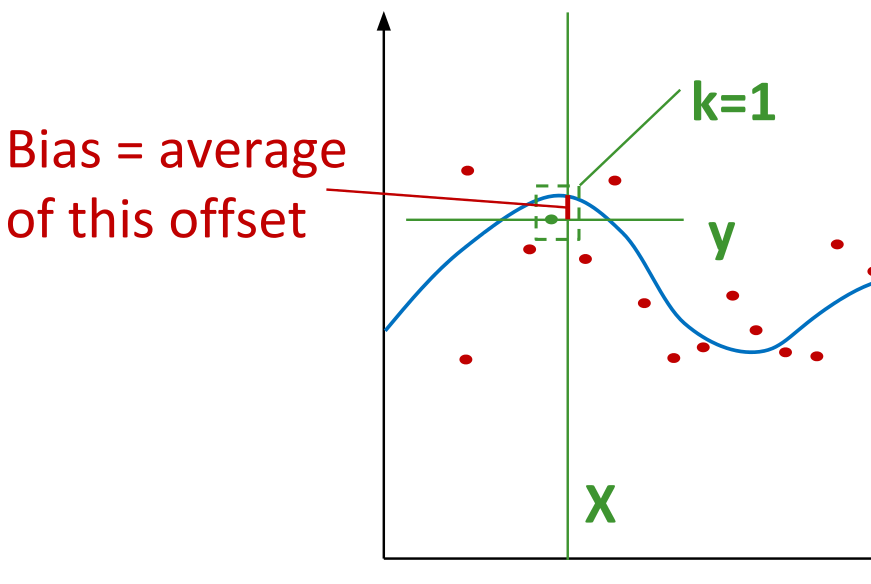
\includegraphics[width=7cm]{img/07/k1_original}}\quad
\subfigure{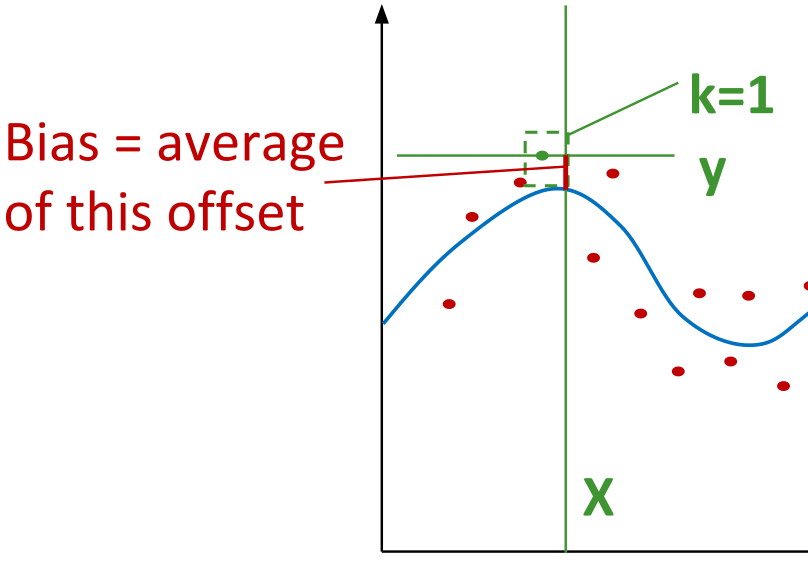
\includegraphics[width=7cm]{img/07/k1_diff}} 
}
\caption{\label{fig:knn_k1} 
Test on two different samples of the kNN algorithm with k=1.
}
\end{figure}

On the other hand if we choose a {\bf large k}, we will see a high bias but low variance. Firgure \ref{fig:knn_k8} shows whats happens with two different samples if we choose a large k.

\begin{figure}[H] %----------- SubGraph ---------------------
\centerline{
\subfigure{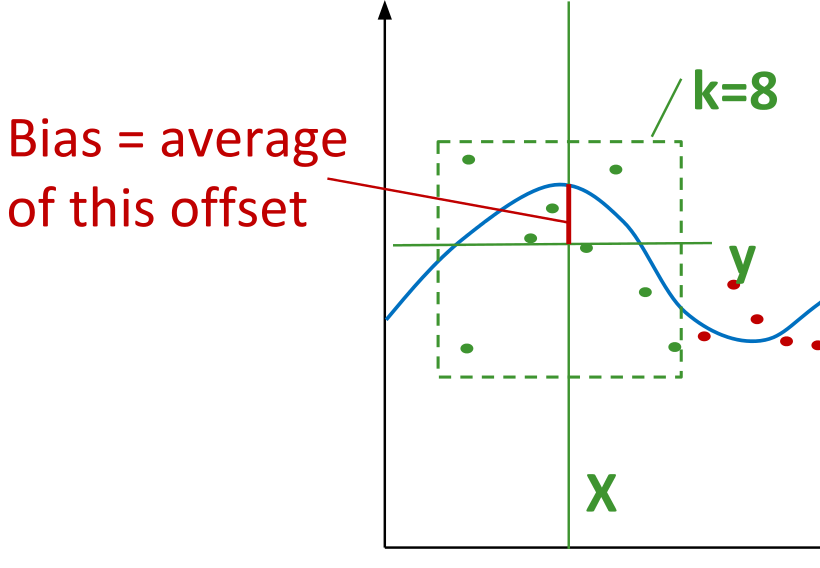
\includegraphics[width=7cm]{img/07/k8_original}}\quad
\subfigure{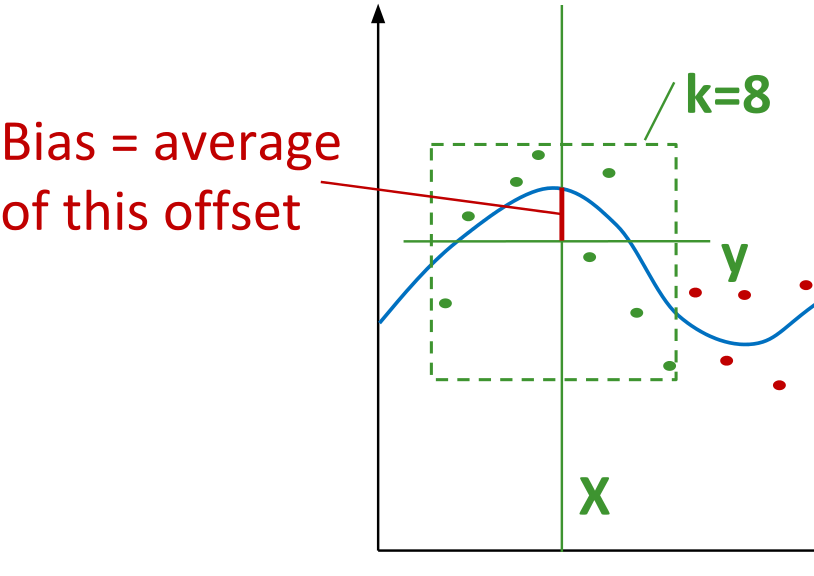
\includegraphics[width=7cm]{img/07/k8_diff}} 
}
\caption{\label{fig:knn_k8} 
Test on two different samples of the kNN algorithm with k=8.
}
\end{figure}

\subsubsection*{In practice}

\begin{description}
 \item[Use cross-validation!] Break data into train, validation and test subsets. For example, you can choose a 60-20-20 \% random split.
 \item[Predict] For each point in the validation set, predict using the k-Nearest neighbors from the training set. Measure the error rate (classification) or the squared error (regression)
 \item[Tune] Try different values of k, and use the one that gives minimum error on the validation set.
 \item[Evaluate] test on the test set to measure performance.
\end{description}

%=============================
\subsubsection{kNN and the curse of dimensionality}

The curse of dimensionality refers to phenomena that occur in high dimensions, from hundreds to millions, that do not occur in low-dimensional space. Data in high dimensions are much sparser than data in low dimensions. That means there are less points that are very close in the feature space. For example, the Euclidean distance scales as $\sqrt{N}$ with $N$ being the dimension. Thus it is quite surprising that kNN works even in high dimensions. 

Luckily data are not random points in a high-dimensional cube. They live in {\bf dense clusters} and near {\bf much lower-dimensional surfaces}. Therefore, we can reduce the feature space in many different way to see the clusters appear.

Even if the Euclidean distance between two point is large they can be very \emph{similar}. For example documents with the same few dominant words (with \href{https://en.wikipedia.org/wiki/Tf-idf}{tf-idf} weighting) are likely to be on the same topic.

\clearpage
%=============================
\subsection{Decision Tree}

Decision Tree (DT) is a basic classifier acting like a \textbf{flow-chart having the following tree structure}  :
\begin{itemize}
	\item \textbf{Decision node}: specifies a test on a single attribute
	\item \textbf{Leaf node}: indicates the value of the target attribute
	\item \textbf{Edge}: split on one attribute
	\item \textbf{Path}: a disjunction of tests to make the final decision
\end{itemize} 

It's constructed following a top-down approach in which, at each node, the data is split on one of their attribute. The prediction are obtained by following the "if-else" statement of each node and is given by the leaves , once the whole tree is traversed (Path). 
\\\\

\textbf{Accuracy} \\
Training accuracy : How many training instances can be correctly classified based on the available data? It is high when the tree is deep/large, or when there is less conflictual instances in the training instances. Never forget that higher training accuracy does not mean good generalization.
Testing accuracy: Given a number of new instances, how many of them can we correctly classify. The only way to score a DT is by counting the number of right elements it predicts on the test set, since the prediction are not "weighted" by a probability of correctness.

\begin{figure}[H] %----------- SubGraph ---------------------
\centerline{
\subfigure{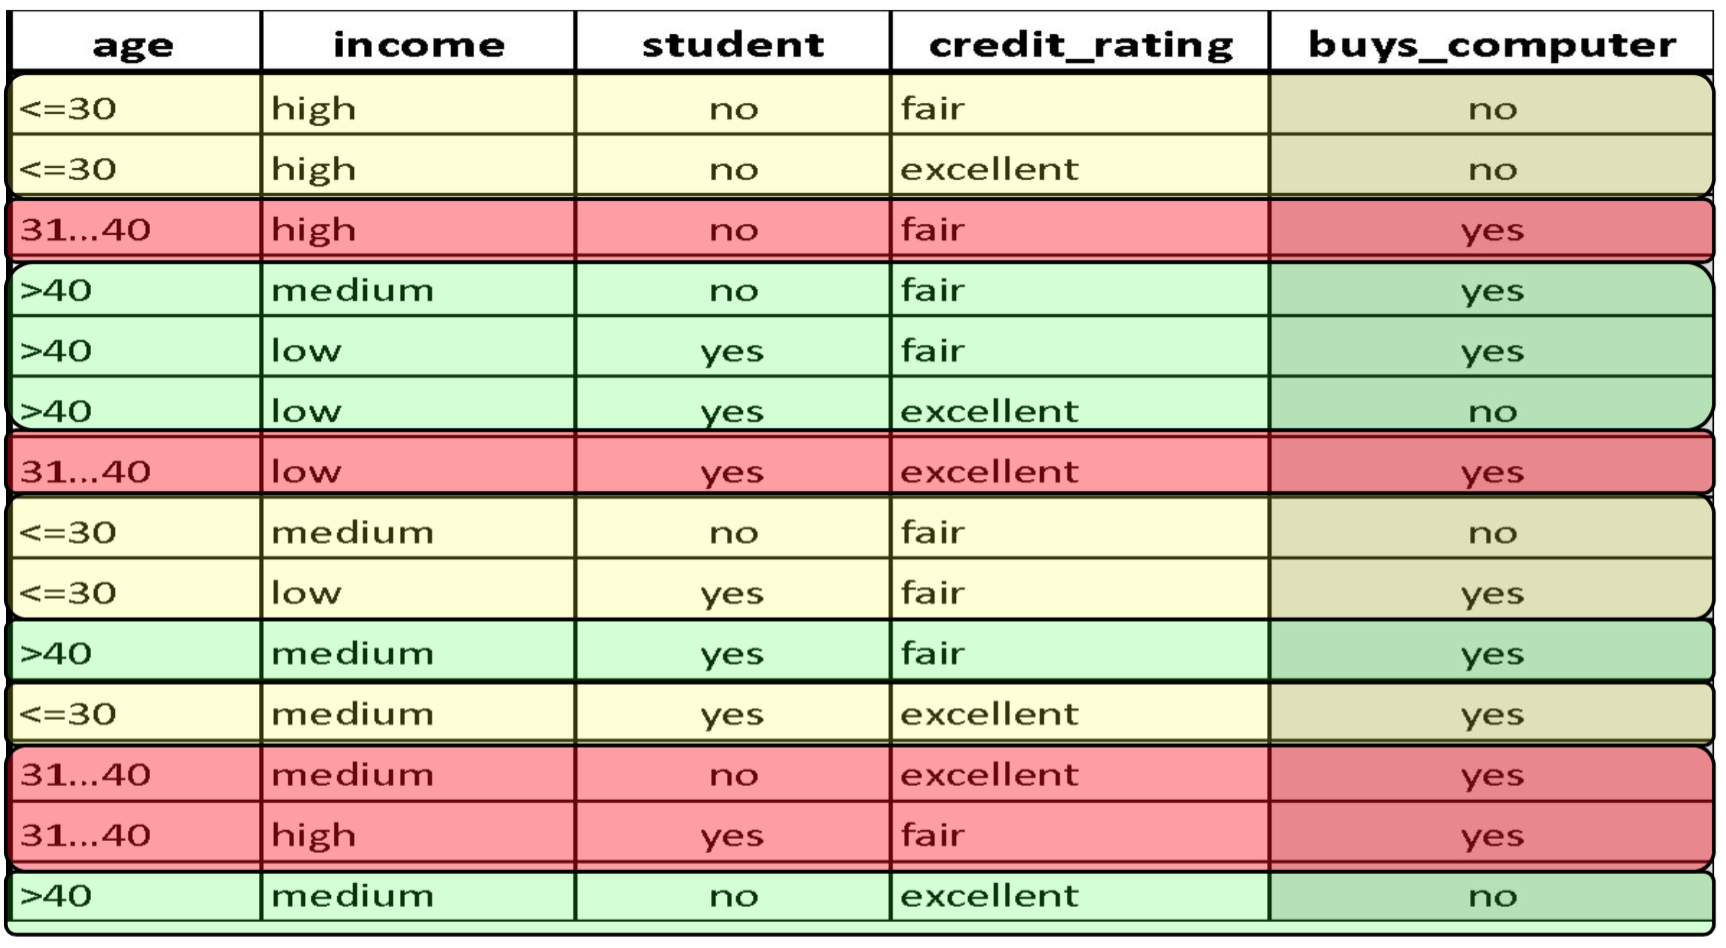
\includegraphics[width=5.5cm]{img/07/DT1}}
\subfigure{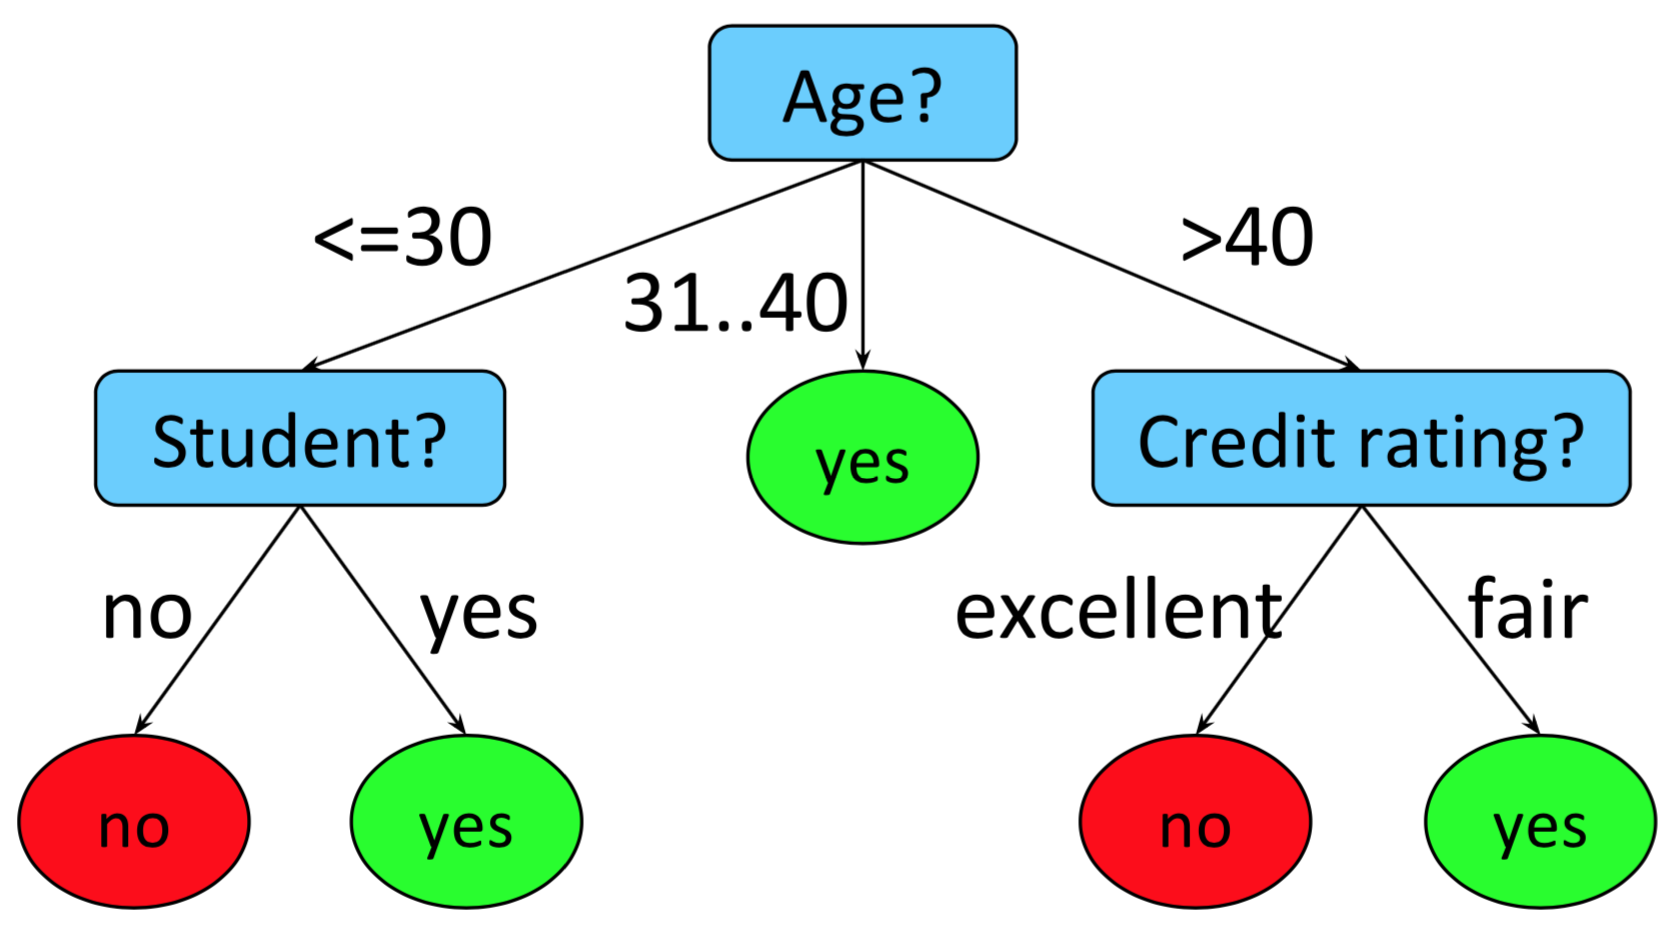
\includegraphics[width=5.5cm]{img/07/DT2}} 
}
\caption{\label{DT} 
Dataset and the Decision Tree related to it.
}
\end{figure}

\textbf{Construction} (Top-down, divide-and-conquer strategy.)
\begin{enumerate}
  \item At the beginning, all the samples are attached to the root.
  \item Recursively, the (sub)sets are partitioned according to their most discriminative attribute (see section \ref{sec:selection} for the ways of selecting of the attributes).
  \item Stop when:
  \begin{itemize}
  	\item A node only contains identically labelled samples, this node becomes a leaf .
  	\item No more attributes are left for splitting, assign the most dominant label to the leaf.
  	\item No more samples left.
  	\item A depth threshold has been defined and has been reached.
  \end{itemize}
\end{enumerate}

The DT will continue to add attributes to its decision process until none are left. As it increases its precision (and then its depth), it starts over fitting the model. A threshold can be defined to stop the construction process earlier and limit this effect. 

\begin{figure}[H]%---------------FIG--------------
 \centering
 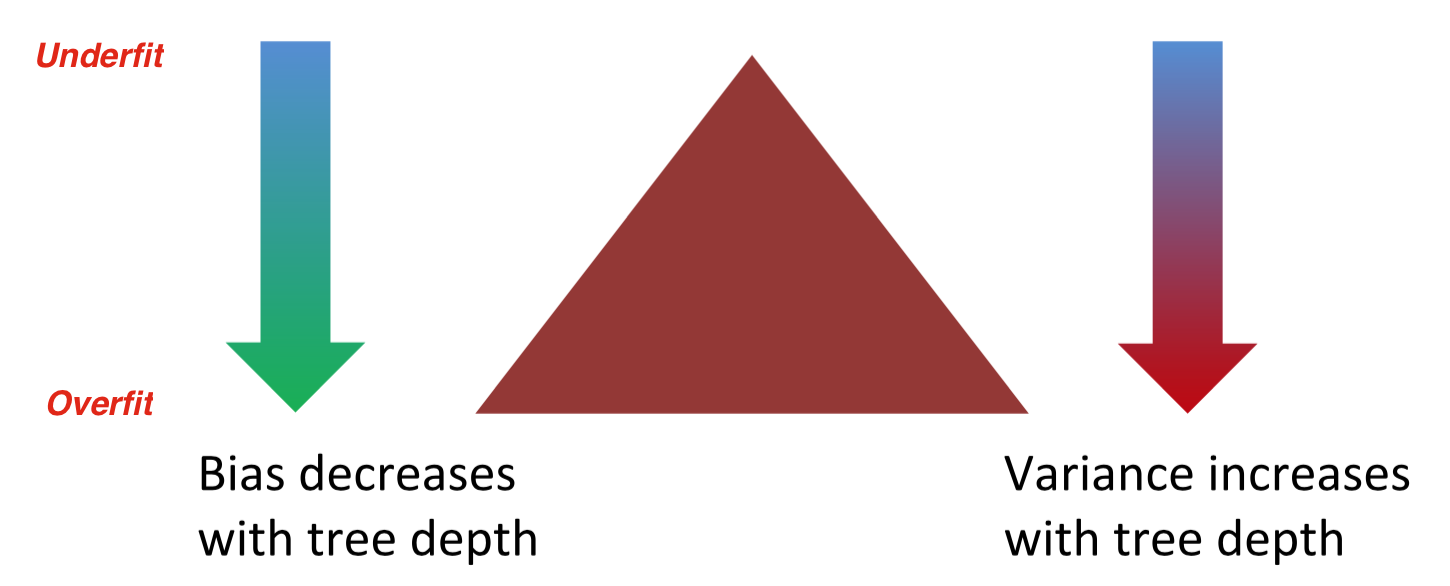
\includegraphics[width=10cm]{./img/07/bias_variance_DT.png}
 \caption{\label{pic:bias_variance_DT.} Bias and variance evolution with DT depth}
\end{figure}

\begin{center} %---------------TAB--------------
\begin{tabular} {| l | l |}
\hline
\bf Pros & \bf Cons \\ \hline
+ A first ML approach ;) & - Sensitive to small perturbation  \\
+ Can be enhanced in RF or BDT  & - Retrained from scratch when new data are coming \\
+ Simple to understand and interpret & - Tend to overfit \\
+ Requires little data preparation \\ 
\hline
\end{tabular}
\end{center}



%=============================
\subsubsection{Attribute selection}
\label{sec:selection}

A big part of the DT model creation relies on choosing the good attribute on which to split the data in each node. One way to achieve this splitting relies on the concept of entropy, which describes the disorder a system and how impactful a feature can be.

For a set $S$ with $P$ positive predictions and $N$ negative ones, its entropy is:
$$
 H(P,N)=-\frac{P}{P+N}\log_2\frac{P}{P+N}-\frac{N}{P+N}\log_2\frac{N}{P+N}
$$
Note that:
\begin{itemize}
 \item If $P \text{ or } N=0 \rightarrow H(P,N)=0$, meaning \textbf{no uncertainty at all}
 \item If $P=N \rightarrow H(P,N)=1$, meaning \textbf{maximum of uncertainty}
\end{itemize}

Entropy of the attribute $A$:
$$
H(A) = \sum_{i} \frac{P_i + N_i}{P + N} * H(P_i, N_i)
$$

Gain obtained by splitting the dataset $S$ by attribute $A$.
$$
Gain(A) = H(P, N) - H(A)
$$

The gain indicates how a split on a certain attribute will influence our data set. The lower the entropy becomes, the greater is the gain, the more \textit{organised} and \textit{certain} become the data set.

The figure \ref{pic:entropy} illustrates how the entropy of an attribute is calculated.

In order to choose how to next split $S$, we compute the gain of each attribute $A$ regarding $S$ and choose the best.

\textbf{Pruning} The construction algorithm aforementioned 	doesn't filter out noise which may lead to over fitting. In order to circumvent this disagreement the Decision tree can be \href{https://en.wikipedia.org/wiki/Pruning_(decision_trees)}{pruned}.


\begin{figure}[H]%---------------FIG--------------
 \centering
 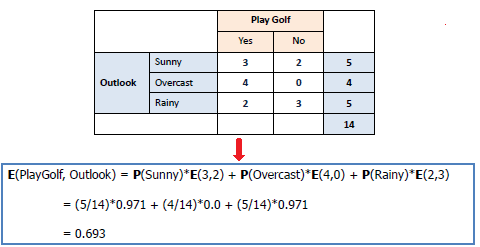
\includegraphics[width=10cm]{./img/07/entropy.png}
 \caption{\label{pic:entropy} Example of entropy calculation.}
\end{figure}






%========================================
\subsubsection{Random Forest}

A common problem when trying to build a model is to select significant features between all the available ones. We tend to think that \textit{the more we have, the better it is}, even knowing the existence of the curse of dimensionality. 

Random Forest exploits this previous idea and tries to automatize the feature selection process by randomly selecting subsets of features.

The main idea of Random Forest algorithm is to grow an arbitrary number of \textbf{Decision Trees}, each one based on a subset of m features, randomly chosen between the total $p$. It's an example of \textbf{weak learners} seen in the Ensemble method. These weak learners have a lower bias (because of lower number of feature).

\textbf{Ensemble methods} can be compared to crowd-sourced machine learning algorithms in the sense that we use a collection of weak learners and combine their results to make a better prediction. There are several different types of ensemble methods : 
\begin{itemize}
	\item \textbf{Bagging :} Train learners in parallel on different samples of the data and then combine the results by voting/averaging for discrete/continuous outputs.
	\item \textbf{Stacking :} A first series of learners is trained on the samples, then a combiner algorithm is trained to make a final prediction using the outputs of the first series of learners.
	\item \textbf{Boosting :} (see next section)  
\end{itemize}

\begin{center} %---------------TAB--------------
\begin{tabular} {| l | l |}
\hline
\bf Pros & \bf Cons \\ \hline
+ Popular & - Not state-of-the-art  \\
+ Easy to implement & - Needs many passes over the data \\
+ Easy to parallelize & - Tend to overfit \\ 
\hline
\end{tabular}
\end{center}

%===============================
\subsubsection{Boosted Decision Trees}
Variant of Random Forests. Instead of performing the training of all DTs independently on a weak subset, train learners on the filtered outputs of other learners. The building of the ensemble is incremental where each new model instance is made to emphasize instances that previous models mis-classified. The accuracy yielded by boosting can be better than bagging but it also tends to overfit the training data. 
This is called \textbf{Boosting}. 
\begin{itemize}
\item Low variance, because of the small trees handling small numbers of features
\item Low bias, reduces by the boosting
\end{itemize}

Opposed to Random Forests that usually trains tens of medium-sized trees, Boosted Decision Trees works on smaller trees in greater numbers.

On the side of performances, even if they show good results, the big drawback of Boosted Decision Trees is their slow execution compared with the parallelized Random Forest.

%===============================
\subsubsection{About model transparency}

A recurrent argument of using Decision Tree (DT) or Random Forest (RF) in industry is their transparency compared to state-of-the-art Deep-Neural-Network (DNN) that are often "black-boxed". This argument must be carefully taken. Even if by their very nature DT are more understandable by a human than DNN, the more features and Trees we had, the more complicated it becomes and the less transparency we have even for DTs. Figure \ref{pic:RF_BT} shows the size of a common industry implementation of RF and BT where there are no more possibilities of human understanding.

\begin{figure}[H]%---------------FIG--------------
 \centering
 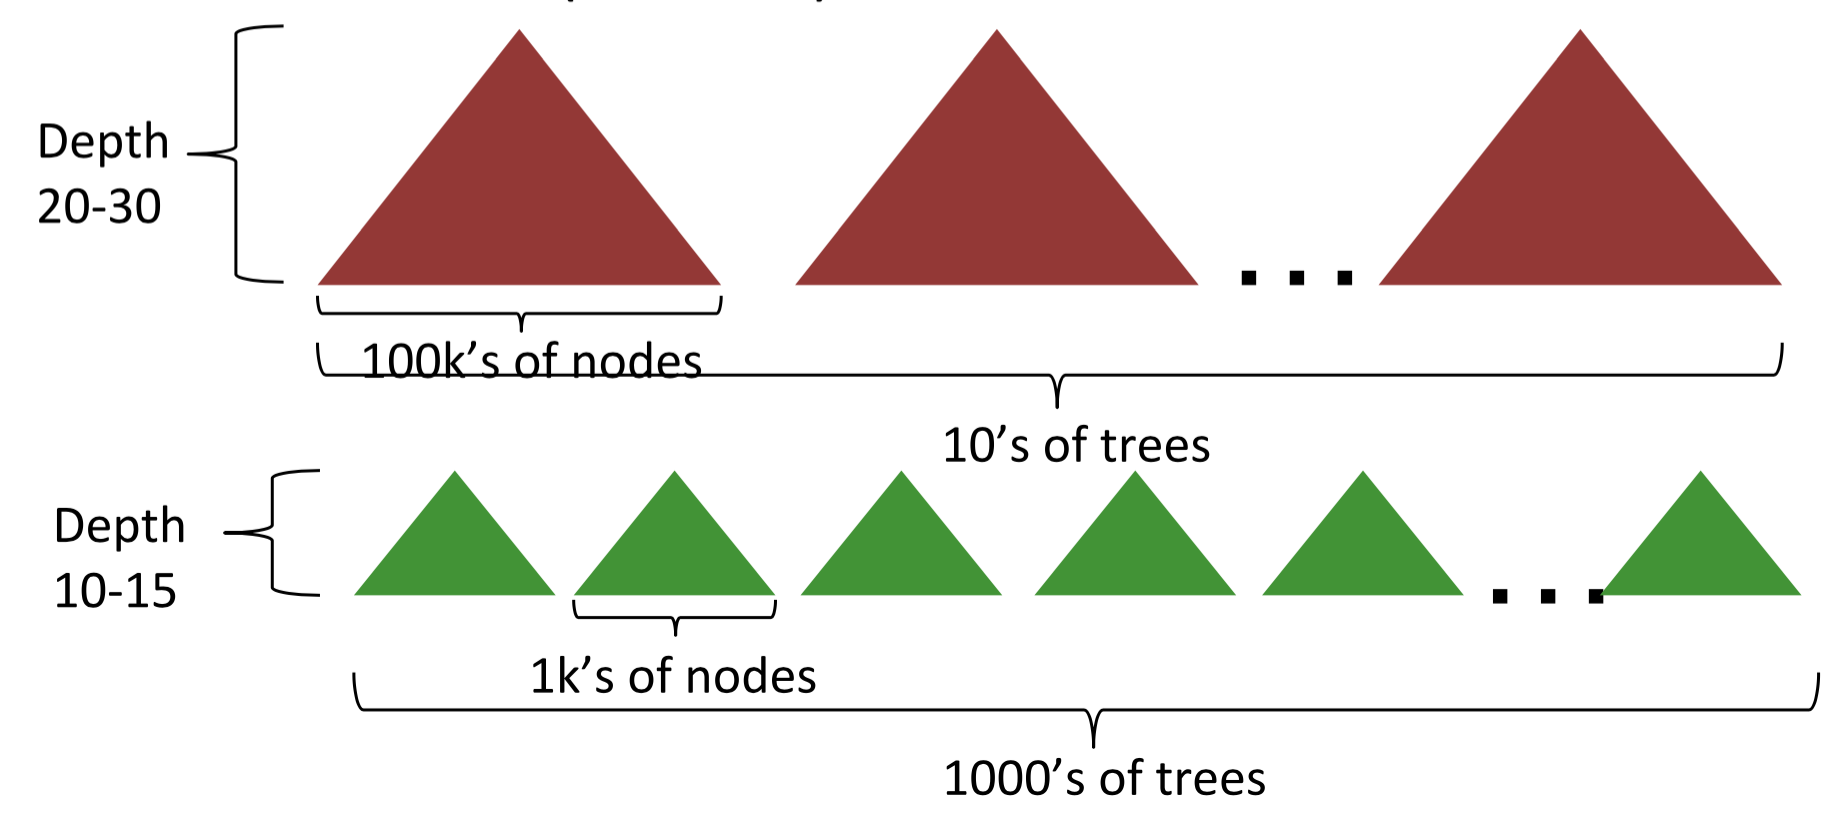
\includegraphics[width=10cm]{./img/07/RF_BT.png}
 \caption{\label{pic:RF_BT.} Standard size of RF and BDT implementations.
 In red: RF with big parallel DT. In green: BDT pipeline with lot of small DT}
\end{figure}


\subsection{Linear Regression}

Linear regression model produces a prediction equation:

$$
\hat{y} = \hat{\beta_0} + \sum\limits_{j=1}^p  X_j \hat{ \beta_j}
$$

or in matrix notation

$$
\hat{y} =X \hat{ \beta}
$$

Where $X = \begin{pmatrix} X_{11} & \cdots & X_{1N} \\ \vdots & \ddots &  \vdots \\ X_{M1} & \cdots & X_{MN} \end{pmatrix}$ is the input data, more precisely, rows of $X$ are distinct observations and columns of $X$ are input features.The $\hat{\beta_j}$ are the coefficients of the model. 

\paragraph{Least Squares Solution}

The most common measure of fit between the line and the data is the \href{https://en.wikipedia.org/wiki/Least_squares}{least-squares} fit because if we start from the hypothesis that the points are the addition of a line with Gaussian noise, the least squares corresponds to the maximum likelihood solution.

\paragraph{Overfitting}

A common mistake that leads to overfitting is to ignore feature selection, in fact having more features doesn't mean getting better results. Therefore it's always a good idea to carefully select features to improve model accuracy. More advanced models of regression include forms of feature control such as \href{https://en.wikipedia.org/wiki/Tikhonov_regularization}{ridge regression} or \href{https://en.wikipedia.org/wiki/Lasso_(statistics)}{Lasso regression} that include embedded regularizers.

\subsubsection{Statistic validation}

As a linear model can be evaluated for every possible existing dataset, it is not enough to compute it, but the existing of a meaningful linear relationship in the data must be determined beforehand.

\paragraph{$R^2$-value}

$R^2$-value describes how much of the total variance is reduced when we include the line as an offset. It computes the distances between the real $y$ and the predicted $\hat{y}$, and compares them with the distance between real $y$ and the mean $\bar{y}$. It's therefore a good indicator on how a line fits our data.

\begin{itemize}
\item if $R^2 = 0$, then there is no difference between the linear model and the trivial mean $\bar{y}$. Then we conclude that there is not any evidence of linear relationship in our dataset and \textbf{we cannot use the model}.
\item if $R^2 = 1$, then the data perfectly aligned on the linear regression line and \textbf{the model is perfect}.
\end{itemize}

\begin{figure}[H]%---------------FIG--------------
 \centering
 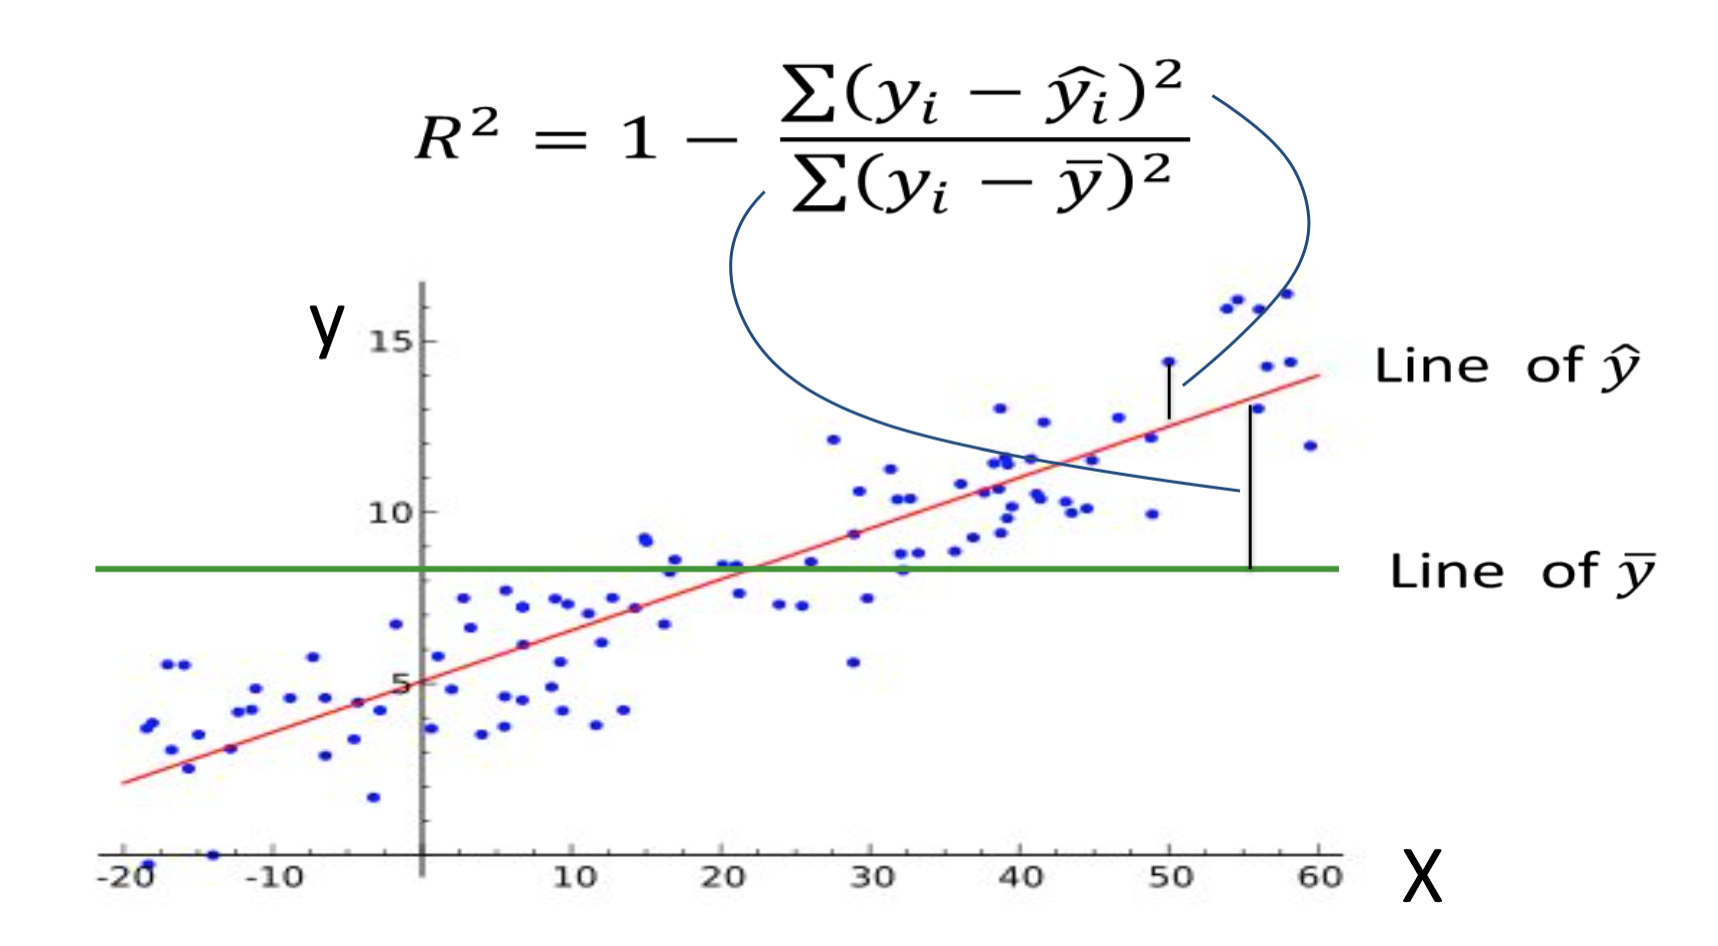
\includegraphics[width=10cm]{./img/07/r_2.png}
 \caption{\label{pic:r_2} Graphical meaning of $R^2$-value.}
\end{figure}


\paragraph{p-value}

From the Distribution of Fisher (F-Distribution) we can derive a p-value which is, as usual, the probability that the observed data validates the null hypothesis which is, in our case, the hypothesis \textit{that there is no linear relationship in the data}. For $p < 0.05$ we conclude, as usual, that it is very unlikely that the data were produced by the null hypothesis and we then accept the hypothesis \textit{the data follows a linear relationship}.














